% The action space: the whole DOS keyboard the API accepts, with the keys the
% game answers picked out, and what the four movement keys do on screen.
% Grid: 1 unit = 1 cm, key pitch 0.63 in both axes, key face 0.56. Layers bottom to top:
% L0 panel, L1 key faces, L2 legends, L3 the isometric inset.
\documentclass[tikz,border=1pt]{standalone}
\usepackage{times}
\usepackage[T1]{fontenc}
\usetikzlibrary{arrows.meta,calc}

\definecolor{ink}{HTML}{1C1C1E}
\definecolor{soft}{HTML}{9C9C9F}
\definecolor{accent}{HTML}{2F6FB0}
\definecolor{accentlt}{HTML}{A8C4DE}
\definecolor{rule}{HTML}{DCDDE0}
\definecolor{dead}{HTML}{F3F4F6}
\definecolor{deadink}{HTML}{B9BBC0}
\definecolor{wash}{HTML}{EEF3F9}

\newcommand{\KP}{0.63}   % key pitch
\newcommand{\KF}{0.56}   % key face

% \key{col}{row}{widthInUnits}{label}{class}
% class: move | alias | act | dead
\newcommand{\key}[5]{%
  \begin{scope}[shift={(#1*\KP, -#2*\KP)}]
    % evaluate first: TikZ would read "1*0.63-..." as a node name
    \pgfmathsetmacro{\w}{#3*\KP-(\KP-\KF)}
    \ifnum\pdfstrcmp{#5}{move}=0
      \fill[accent,rounded corners=1.1pt] (0,0) rectangle (\w,\KF);
      \node[font=\sffamily\tiny\bfseries,text=white] at (\w/2,\KF/2) {#4};
    \else\ifnum\pdfstrcmp{#5}{alias}=0
      \fill[accentlt,draw=accent,line width=0.35pt,rounded corners=1.1pt] (0,0) rectangle (\w,\KF);
      \node[font=\sffamily\tiny,text=ink] at (\w/2,\KF/2) {#4};
    \else\ifnum\pdfstrcmp{#5}{act}=0
      \fill[white,draw=ink,line width=0.6pt,rounded corners=1.1pt] (0,0) rectangle (\w,\KF);
      \node[font=\sffamily\tiny\bfseries,text=ink] at (\w/2,\KF/2) {#4};
    \else
      \fill[dead,draw=rule,line width=0.3pt,rounded corners=1.1pt] (0,0) rectangle (\w,\KF);
      \node[font=\sffamily\tiny,text=deadink] at (\w/2,\KF/2) {#4};
    \fi\fi\fi
  \end{scope}}

\begin{document}
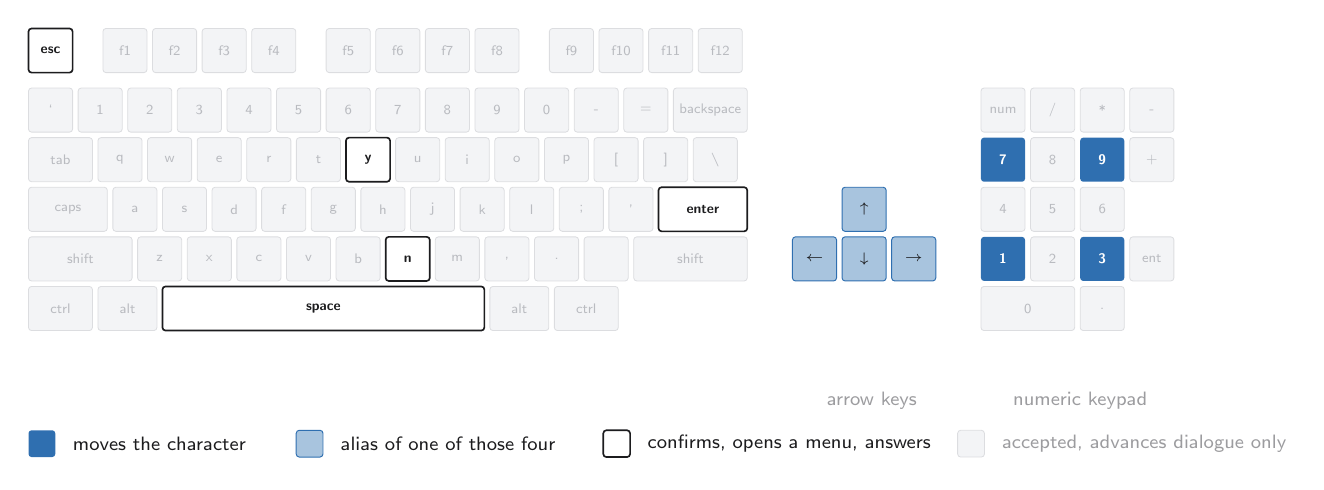
\begin{tikzpicture}[font=\sffamily,>={Stealth[length=2.4mm,width=1.7mm]}]

% ---------------- L1: main block -------------------------------------------
\key{0}{0}{1}{esc}{act}
\foreach \i/\f in {1.5/1,2.5/2,3.5/3,4.5/4,6/5,7/6,8/7,9/8,10.5/9,11.5/10,12.5/11,13.5/12}
  {\key{\i}{0}{1}{f\f}{dead}}

\foreach \i/\c in {0/`,1/1,2/2,3/3,4/4,5/5,6/6,7/7,8/8,9/9,10/0,11/-,12/=}
  {\key{\i}{1.2}{1}{\c}{dead}}
\key{13}{1.2}{1.6}{backspace}{dead}

\key{0}{2.2}{1.4}{tab}{dead}
\foreach \i/\c in {1.4/q,2.4/w,3.4/e,4.4/r,5.4/t,6.4/y,7.4/u,8.4/i,9.4/o,10.4/p,11.4/[,12.4/],13.4/\textbackslash}
  {\key{\i}{2.2}{1}{\c}{dead}}

\key{0}{3.2}{1.7}{caps}{dead}
\foreach \i/\c in {1.7/a,2.7/s,3.7/d,4.7/f,5.7/g,6.7/h,7.7/j,8.7/k,9.7/l,10.7/;,11.7/'}
  {\key{\i}{3.2}{1}{\c}{dead}}
\key{12.7}{3.2}{1.9}{enter}{act}

\key{0}{4.2}{2.2}{shift}{dead}
\foreach \i/\c in {2.2/z,3.2/x,4.2/c,5.2/v,6.2/b}
  {\key{\i}{4.2}{1}{\c}{dead}}
\key{7.2}{4.2}{1}{n}{act}
\foreach \i/\c in {8.2/m,9.2/{,},10.2/.,11.2//}
  {\key{\i}{4.2}{1}{\c}{dead}}
\key{12.2}{4.2}{2.4}{shift}{dead}

\key{0}{5.2}{1.4}{ctrl}{dead}
\key{1.4}{5.2}{1.3}{alt}{dead}
\key{2.7}{5.2}{6.6}{space}{act}
\key{9.3}{5.2}{1.3}{alt}{dead}
\key{10.6}{5.2}{1.4}{ctrl}{dead}
% y sits in the letter row; drawn last so its outline is not overpainted
\key{6.4}{2.2}{1}{y}{act}

% ---------------- L1: arrows and numpad ------------------------------------
\begin{scope}[shift={(15.4*\KP,0)}]
  \key{1}{3.2}{1}{$\uparrow$}{alias}
  \key{0}{4.2}{1}{$\leftarrow$}{alias}
  \key{1}{4.2}{1}{$\downarrow$}{alias}
  \key{2}{4.2}{1}{$\rightarrow$}{alias}
  \node[font=\sffamily\scriptsize,text=soft,anchor=north] at (1.6*\KP,-6.25*\KP) {arrow keys};
\end{scope}

\begin{scope}[shift={(19.2*\KP,0)}]
  \key{0}{1.2}{1}{num}{dead} \key{1}{1.2}{1}{/}{dead}
  \key{2}{1.2}{1}{*}{dead}   \key{3}{1.2}{1}{-}{dead}
  \key{0}{2.2}{1}{7}{move}   \key{1}{2.2}{1}{8}{dead}
  \key{2}{2.2}{1}{9}{move}   \key{3}{2.2}{1}{+}{dead}
  \key{0}{3.2}{1}{4}{dead}   \key{1}{3.2}{1}{5}{dead}
  \key{2}{3.2}{1}{6}{dead}
  \key{0}{4.2}{1}{1}{move}   \key{1}{4.2}{1}{2}{dead}
  \key{2}{4.2}{1}{3}{move}   \key{3}{4.2}{1}{ent}{dead}
  \key{0}{5.2}{2}{0}{dead}   \key{2}{5.2}{1}{.}{dead}
  \node[font=\sffamily\scriptsize,text=soft,anchor=north] at (2*\KP,-6.25*\KP) {numeric keypad};
\end{scope}

% ---------------- L2: legend -----------------------------------------------
\begin{scope}[shift={(0,-7.75*\KP)}]
  \fill[accent,rounded corners=1.1pt] (0,0) rectangle (0.34,0.34);
  \node[font=\sffamily\scriptsize,text=ink,anchor=west] at (0.44,0.17) {moves the character};
  \fill[accentlt,draw=accent,line width=0.35pt,rounded corners=1.1pt] (3.4,0) rectangle (3.74,0.34);
  \node[font=\sffamily\scriptsize,text=ink,anchor=west] at (3.84,0.17) {alias of one of those four};
  \fill[white,draw=ink,line width=0.6pt,rounded corners=1.1pt] (7.3,0) rectangle (7.64,0.34);
  \node[font=\sffamily\scriptsize,text=ink,anchor=west] at (7.74,0.17) {confirms, opens a menu, answers};
  \fill[dead,draw=rule,line width=0.3pt,rounded corners=1.1pt] (11.8,0) rectangle (12.14,0.34);
  \node[font=\sffamily\scriptsize,text=soft,anchor=west] at (12.24,0.17) {accepted, advances dialogue only};
\end{scope}

\end{tikzpicture}
\end{document}
